\documentclass[10pt,final,oneside]{amsbook}
\usepackage[margin=100pt,includehead]{geometry}
\usepackage[cat,garamondx,secnum]{trinh-m-q_15_00}

\usepackage{stmaryrd, tikz-cd}

%	http://tex.stackexchange.com/a/29659

\makeatletter 
\renewenvironment{proof}[1][\proofname] 
{ 	
	\par\pushQED{\qed}\normalfont\topsep6\p@\@plus6\p@\relax\trivlist\itemindent\normalparindent
	\item[\hskip\labelsep\itshape#1\@addpunct{.}]\ignorespaces
}
{
	\popQED\endtrivlist\@endpefalse
}
\makeatother

\numberwithin{equation}{section}

%	http://chat.stackexchange.com/transcript/41/2013/9/13/0-24

\makeatletter
\newcommand{\xmapsfrom}[2][]
{	
	\ext@arrow3095\leftarrowfill@{#1}{#2}\mapsfromchar
}
\makeatother

\newcommand{\cl}{\mathrm{cl}}
\newcommand{\gr}{\mathrm{gr}}

\newcommand{\Aff}{\mathsf{Aff}}
\newcommand{\LRS}{\mathsf{LRS}}
\newcommand{\SHom}{{\mathcal{H}\mathit{om}}}
\newcommand{\SEnd}{{\mathcal{E}\mathit{nd}}}

\begin{document}

\frontmatter

%	Title block

\title{\MakeUppercase{Algebraic Geometry}}
%	\dedicatory{}
%	\subjclass[2010]{}
%	\keywords{}
%		\thanks{}

%	Author block(s)

\author{Minh-Tam Trinh}

\maketitle
\tableofcontents

%--------------------------------------------------------------------------

\mainmatter

\chapter*{Conventions}

The symbol $\simeq$ always denotes a functorial isomorphism.
We reserve the symbol $=$ for definitions and purely set-theoretic computations.
We write $\Ring$ (resp., $\Set$, $\Top$) for the category of rings (resp., sets, topological spaces).

All rings are commutative unital, and all ring morphisms are unital.
We allow the possibility that $1 = 0$, i.e., the ``zero ring'' is a ring.
If $A$ is a ring, then we write $\Mod_A$ for the category of $A$-modules.
For all local rings $A$, we write $\fr{m}_A$ (resp., $\kappa_A$) for the maximal ideal (resp., residue field) of $A$.
For all integral domains $A$, we write $\frak{K}_A$ for the field of fractions of $A$.

\setcounter{chapter}{-1}
%%%
%%%
%%%
\chapter{Ringed Spaces}

\subsection{}

Assuming the reader's familiarity with commutative algebra and sheaves, we find it logical to discuss \emph{ringed spaces} and their sheaves before we discuss rings themselves.
Ringed spaces encompass not only the objects of algebraic geometry, but topological and differentiable manifolds as well; in this sense, they are actually prior to our subject.

\section{Definition}

\subsection{}

A \emph{ringed space} is a pair $(X, \cal{O}_X)$, where $X$ is a topological space and $\cal{O}_X$ is a sheaf of rings on $X$, called its \emph{structure sheaf}.
We abbreviate by writing $X$ in place of $(X, \cal{O}_X)$ when there is no ambiguity.
Similarly, we write $\cal{O}_x$ in place of $\cal{O}_{X, x}$.
A \emph{ringed-space morphism} $Y \to X$ is a pair $(\eta, \eta^\#)$ such that $\eta : Y \to X$ is a continuous map and $\eta^\# : \cal{O}_X \to \eta_\ast \cal{O}_Y$ is a morphism of sheaves on $X$.
We write $\eta$ in place of $(\eta, \eta^\#)$ when there is no ambiguity.
If $\eta : Y \to X$ is an ringed-space morphism, then for all $y \in  Y$, there is an induced morphism $\eta_y^\# : \cal{O}_{\eta(y)} \to \cal{O}_{y}$, given by either of the possible compositions of arrows in the following commutative diagram:
\begin{equation}
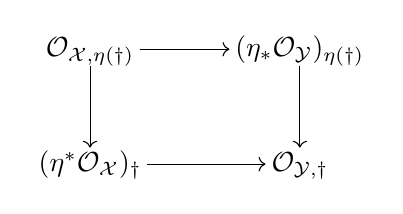
\begin{tikzpicture}[baseline=(current  bounding  box.center)]
\tikzstyle{every node}=[fill=white,  inner sep=2pt]
\matrix (m)
[	matrix of math nodes,
	row sep 		=	3em,
	column sep 	=	3em,
	text height	=	1.5ex,
	text depth	=	0.25ex
]
{ 		\cal{O}_{X, \eta(y)}		&(\eta_\ast \cal{O}_Y)_{\eta(y)}	\\
		(\eta^\ast\cal{O}_X)_y	&\cal{O}_{Y, y}\\
};
\path[->, font=\small]
(m-1-1) edge 	(m-1-2)
(m-1-1) edge 	(m-2-1)
(m-1-2) edge 	(m-2-2)
(m-2-1) edge 	(m-2-2);
\end{tikzpicture}
\end{equation}
If $\eta : Y \to X$ and $\theta : X \to W$ are ringed-space morphisms, then we define their composition to be the morphism $\theta \circ \eta : Y \to W$ given on the topological spaces by the usual composition and given on the structure sheaves by
\begin{align}
\theta_\ast\eta^\# \circ \theta^\# : \cal{O}_W \to \theta_\ast \cal{O}_X \to \theta_\ast \eta_\ast \cal{O}_Y \simeq (\theta \circ \eta)_\ast \cal{O}_Y.
\end{align}
In this way, there is a well-defined category of ringed spaces.

%%%
\section{Sheaves}

\subsection{}

Throughout the rest of this chapter, let $X$ be a ringed space.
We write $\Ab_X$ for the category of sheaves of abelian groups on $X$.
An \emph{$\cal{O}_X$-module} is a pair $(\cal{F}, \rho)$, where $\cal{F}$ is an object of $\Ab_X$ and $\rho$ is an $\cal{O}_X$-action on $\cal{F}$, i.e., a morphism $\cal{O}_X \to \SEnd(\cal{F})$.
Explicitly, $\rho$ is equivalent to giving $\cal{F}(U)$ the structure of an $\cal{O}_X(U)$-module, for all open $U$, such that these local actions commute with restriction maps.
We write $\cal{F}$ in place of $(\cal{F}, \rho)$ when there is no ambiguity.
An \emph{$\cal{O}_X$-module morphism $\cal{F} \to \cal{G}$} is a sheaf morphism that is $\cal{O}_X$-linear, meaning $\cal{F}(U) \to \cal{G}(U)$ is $\cal{O}_X(U)$-linear for all $U$.
We write $\Mod_X$ for the category of $\cal{O}_X$-modules.
An \emph{$\cal{O}_X$-algebra} is a monoid object in $\Mod_X$.

\begin{prop}
$\Mod_X$ is a complete and cocomplete abelian category.
Moreover, the forgetful functor $\Mod_X \to \Ab_X$ preserves limits and colimits.
\end{prop}

\begin{proof}
Recall that the underlying presheaf of a limit of $\Ab$-valued sheaves is the limit of the underlying presheaves.
Recall that a colimit of $\Ab$-valued sheaves is the sheafification of the colimit of the underlying presheaves.
Finally, if $\cal{F}$ is an $\Ab$-valued presheaf, then any $\cal{O}_X$-action $\cal{O}_X \to \SEnd(\cal{F})$ induces a uniquely compatible $\cal{O}_X$-action $\cal{O}_X \to \SEnd(\cal{F}^\#)$ via the morphisms $\End(\cal{F}|_U) \to \End(\cal{F}|_U^\#) \simeq \End(\cal{F}^\#|_U)$ induced by the functoriality of sheafification.
The desired statements follow.
\end{proof}

For all $\cal{O}_X$-modules $\cal{F}, \cal{G}$, we abbreviate by writing $\Hom_{\cal{O}_X}(\cal{F}, \cal{G})$ in place of $\Hom_{\Mod_X}(\cal{F}, \cal{G})$.
The \emph{tensor product of $\cal{F}$ and $\cal{G}$ over $\cal{O}_X$} is the $\cal{O}_X$-module $\cal{F} \otimes_{\cal{O}_X} \cal{G}$ whose underlying $\Ab_X$ object is the sheafification of the presheaf that sends 
\begin{align}
U \mapsto \cal{F}(U) \otimes_{\cal{O}_X(U)} \cal{G}(U).
\end{align}
The operation $\otimes_{\cal{O}_X}$ makes $\Mod_X$ into a monoidal category, for which the unit object is $\cal{O}_X$.

The \emph{$\cal{O}_X$-module hom $\cal{F} \to \cal{G}$} is the $\cal{O}_X$-module $\SHom_{\cal{O}_X}(\cal{F}, \cal{G})$ whose underlying $\Ab_X$ object is the subsheaf of $\SHom(\cal{F}, \cal{G})$ that sends 
\begin{align}
U \mapsto \Hom_{\cal{O}_X|_U}(\cal{F}|_U, \cal{G}|_U).
\end{align}
We write $\SEnd_{\cal{O}_X}(\cal{F}) = \SHom_{\cal{O}_X}(\cal{F})$.

We say that an $\cal{O}_X$-module $\cal{E}$ is \emph{free} iff it is isomorphic to a direct sum of copies of $\cal{O}_X$, and \emph{locally free} iff it is locally isomorphic to a free $\cal{O}_X$-module.
In the latter case, we say that $\cal{E}$ has rank $r$ over $U$ iff $\cal{E}|_U \simeq \cal{O}_X^r|_U$.
Moreover, we define the \emph{dual of $\cal{E}$} to be
\begin{align}
\cal{E}^\vee = \SHom_{\cal{O}_X}(\cal{E}, \cal{O}_X).
\end{align}
While $\SHom_{\cal{O}_X}$ does \emph{not} form an internal-hom of $\Mod_X$, it behaves as such for locally-free $\cal{O}_X$-modules of finite rank:

\begin{prop}
Let $\cal{E}$ be a locally-free $\cal{O}_X$-module of finite rank.
Then the following hold:
\begin{enumerate}
\item 	\emph{Rigidity}.
			$\cal{E}^{\vee\vee} \simeq \cal{E}$.
\item 	\emph{Sheafified tensor-hom adjunction}.
			If $\cal{F}, \cal{G}$ are $\cal{O}_X$-modules, then
			\begin{align}
			\SHom_{\cal{O}_X}(\cal{F} \otimes_{\cal{O}_X} \cal{E}, \cal{G})
			\simeq 	
			\SHom_{\cal{O}_X}(\cal{F}, \SHom_{\cal{O}_X}(\cal{E},\cal{G})).
			\end{align}
\end{enumerate}
\end{prop}

\begin{proof}
Since it suffices to check the isomorphisms above locally, we reduce to the case where $\cal{E}$ is free.
In this setting, the commutative algebra suggests natural morphisms that, by the freeness of $\cal{E}$, induce isomorphisms at the level of stalks.
\end{proof}

\subsection{}

Let $\eta : Y \to X$ be a ringed-space morphism.
If $\cal{G}$ is an $\cal{O}_Y$-module, then the \emph{direct image of $\cal{G}$ under $\eta$} is the $\cal{O}_X$-module formed by $\eta_\ast \cal{G}$ under the composition action 
\begin{align}
\cal{O}_X \xrightarrow{\eta^\#} \eta_\ast \cal{O}_Y \to \eta_\ast \SEnd(\cal{G}) \simeq \SEnd(\eta_\ast \cal{G}).
\end{align}
If $\cal{F}$ is an $\cal{O}_X$-module, then the \emph{inverse image of $\cal{F}$ under $\eta$} is the $\cal{O}_Y$-module formed by 
\begin{align}
\eta^\ast \cal{F} = \eta^{-1}\cal{F} \otimes_{\eta^{-1}\cal{O}_X} \cal{O}_Y,
\end{align}
where $\cal{O}_Y$ forms an $\eta^{-1}\cal{O}_X$-algebra via the pullback-pushout adjunction for sheaves of rings.

\begin{prop}[Pullback-Pushout Adjunction]
If $\eta : Y \to X$ is a ringed-space morphism, then $(\eta^\ast, \eta_\ast)$ is an adjoint pair:
If $\cal{F}$ is an $\cal{O}_X$-module and $\cal{G}$ is an $\cal{O}_Y$-module, then
\begin{align}
\Hom_{\cal{O}_Y}(\eta^\ast \cal{F}, \cal{G}) 
\simeq	
\Hom_{\cal{O}_X}(\cal{F}, \eta_\ast\cal{G}).
\end{align}
\end{prop}

\begin{proof}
Imitate the proof of the pullback-pushout adjunction for sheaves of abelian groups.
\end{proof}

\begin{prop}[Projection Formula]
Let $\eta : Y \to X$ be a ringed-space morphism.
If $\cal{E}$ is a locally-free $\cal{O}_X$-module of finite rank and $\cal{F}$ is an $\cal{O}_Y$-module, then
\begin{align}
\eta_\ast(\cal{F} \otimes_{\cal{O}_Y} \eta^\ast \cal{E})
\simeq		
\eta_\ast \cal{F} \otimes_{\cal{O}_X} \cal{E}.
\end{align}
\end{prop}

\begin{proof}
Since it suffices to check the isomorphism locally, we can assume $\cal{E}$ is free.
If $\cal{E} \simeq \cal{O}_X^r$, then $\eta^\ast \cal{E} \simeq \cal{O}_Y^r$.
In this case, $\eta_\ast(\cal{F} \otimes_{\cal{O}_Y} \eta^\ast \cal{E}) \simeq \eta_\ast (\cal{F}^r) \simeq (\eta_\ast \cal{F})^r \simeq \eta_\ast \cal{F} \otimes_X \cal{E}$.
\end{proof}

%%%
\section{Sheaf Cohomology}

\subsection{}

\subsection{}


%%%
%%%
%%%
\chapter{Affine Schemes}

\subsection{}

The heart of modern algebraic geometry is a full and faithful anti-embedding of the category of rings into a category of certain ringed spaces called \emph{locally-ringed spaces}.
The objects in the essential image are called \emph{affine schemes}.
The correspondence between rings and affine schemes is as follows:
Prime ideals correspond to points; ideals correspond to closed sets; ring elements correspond to functions.
Later, we will define schemes to be the locally-ringed spaces that are locally isomorphic to affine schemes.

%%%
\section{The Zariski Topology}

%		We first describe its underlying topological space; then, we define locally-ringed spaces, and equip $\Spec A$ with a sheaf that makes it a locally-ringed space.

\subsection{}

Throughout this chapter, let $A$ be a ring.
The affine scheme associated to $A$ will be called the \emph{spectrum of $A$} and denoted $\Spec A$.
We define the underlying set of $\Spec A$ to be the set of prime ideals of $A$.
For all $T \subseteq A$, let $Z(T) = \{\fr{p} \in \Spec A : \fr{p} \supseteq T\}$.
For all $f \in A$, we abbreviate by writing $Z(f)$ in place of $Z(\{f\})$.
Let $D(f) = \{\fr{p} \in \Spec A : \fr{p} \not\ni f\}$.

\begin{prop}\label{Zariski}\mbox{}
\begin{enumerate}
\item 	If $T_1, \ldots, T_n \subeq A$, then $Z(T_1) \cup \cdots \cup Z(T_n) = Z(T_1 \cap \cdots \cap T_n) = Z(T_1 \cdots T_n)$.
\item 	If $\{T_i\}_i$ is an arbitrary collection of subsets of $A$, then $\bigcap_i Z(T_i) = Z(\bigcup_i T_i)$.
\item 	If $f_1, \ldots, f_n \in A$, then $D(f_1) \cap \cdots \cap D(f_n) = D(f_1\cdots f_n)$.
\item 	\emph{Prime avoidance}.
			If $\fr{a} \normal A$ and $\fr{p}_1, \ldots, \fr{p}_n \notin Z(\fr{a})$, then $\fr{p}_1, \ldots, \fr{p}_n \in D(f)$ for some $f \in \fr{a}$.
\end{enumerate}
\end{prop}

\begin{proof}
(4) is \cite[Prop.~1.11(1)]{AM}.
To show the other parts:
\begin{enumerate}
\item 	We have $Z(T_1) \cup \ldots \cup Z(T_n) \subeq Z(T_1 \cap \cdots \cap T_n) \subeq  Z(T_1 \ldots T_n)$ by definition.
			It remains to show that if $\fr{p} \not\supseteq T_i$ for all $i$, then $\fr{p} \not\supseteq T_1\cdots T_n$.
			Indeed, if $f_i \in T_i \setminus \fr{p}$ for all $i$, then $f_1 \cdots f_n \in T_1\cdots T_n \setminus \fr{p}$, as needed.
\item 	By definition.
\item 	Follows from (1) because $D(f) = \Spec A \setminus Z(f)$.\qedhere
\end{enumerate}
\end{proof}

By Prop.~\ref{Zariski}(1)-(2), there is a topology on $\Spec A$, which we call the \emph{Zariski topology}, in which the closed sets take the form $Z(\fr{a})$ for $\fr{a} \normal A$. By Prop.~\ref{Zariski}(3), the sets $D(f)$ form a basis of open neighborhoods, called \emph{distinguished opens}, as $f$ runs through $A$.

\begin{prop}\label{Contraction}
Let $\phi : A \to B$ be a ring morphism.
Let $\eta$ be the set-theoretic map $\Spec B \to \Spec A$ given by contraction of prime ideals along $\phi$.
\begin{enumerate}
\item 	If $\fr{a} \normal A$, then $\eta^{-1}(Z(\fr{a})) = Z(\phi(\fr{a}))$.
\item 	If $f \in A$, then $\eta^{-1}(D(f)) = D(\phi(f))$.
\item 	If $\fr{b} \normal B$, then $\eta(Z(\fr{b}))$ is dense in $Z(\phi^{-1}(\fr{b}))$.
\end{enumerate}
\end{prop}

\begin{proof}
\cite[Ex.~1.22]{AM}.
\end{proof}

By Prop.~\ref{Contraction}(1)-(2), the map that sends a ring to its spectrum extends to a functor $\Ring \to \Top$, that on morphisms, sends $\phi$ to contraction of prime ideals along $\phi$.

\subsection{}

The functor $\Ring \to \Top$ is not an embedding:
We will show that, as a map on objects, it ignores the data of nilpotent elements.
For all $\fr{a} \normal A$, we write $r(\fr{a})$ for the radical of $\fr{a}$.
We write $\fr{n}(A)$ for the nilradical of $A$, that is to say, for $r(0)$.

\begin{prop}
If $\fr{a} \normal A$, then $r(\fr{a}) = \bigcap_{\fr{p} \in Z(\fr{a})} \fr{p}$.
\end{prop}

\begin{proof}
Since $A \surject A/\fr{a}$ induces an inclusion-preserving bijection of ideals by \cite[1.1]{AM}, it suffices to do the case $\fr{a} = 0$, i.e., to show that $\fr{n}(A) = \bigcap_{\fr{p} \in \Spec A} \fr{p}$.
This is \cite[1.8]{AM}.
\end{proof}

\begin{cor}\label{SpecNullstellensatz}
There is an inclusion-reversing bijection between radical ideals $\fr{r} \normal A$ and closed subsets $Z\subeq \Spec A$, defined by:
\begin{align}
\begin{array}{rcl}
\fr{r}										&\mapsto 		&Z(\fr{r})\\
\bigcap_{\fr{p} \in Z} \fr{p}	&\mapsfrom		&Z	
\end{array}
\end{align}
\end{cor}

\begin{proof}
The proposition says the composition $\fr{r} \mapsto Z(\fr{r}) \mapsto \smash{\bigcap_{\fr{p} \in Z(\fr{r})}} \fr{p}$ is an identity map.
It also implies that $Z(\fr{a}) \subeq Z(\fr{r}(\fr{a}))$, whence $Z(\fr{a}) = Z(\fr{r}(\fr{a})) = Z(\smash{\bigcap_{\fr{p} \in Z(\fr{a})}} \fr{p})$.
Thus the reverse composition is also an identity map.
\end{proof}

\begin{cor}\label{EmptyOrAll}\mbox{}
\begin{enumerate}
\item 	$Z(A) = \emptyset$.
\item 	$Z(\fr{a}) = \Spec A$ if and only if $\fr{a} \subeq \fr{n}(A)$.
\item 	$D(f) = \Spec A$ if and only if $f \in A^\times$.
\item 	$D(f) = \emptyset$ if and only if $f \in \fr{n}(A)$.
\end{enumerate}
\end{cor}

\subsection{}

Even though the map from rings into topological spaces is not injective, various topological properties of $\Spec A$ and its subsets reflect algebraic properties of $A$ and its ideals.

\begin{prop}
$\Spec A$ is always Kolmogorov ($T_0$) and quasicompact.
\end{prop}

\begin{proof}
To show that $\Spec A$ is Kolmogorov:
If $\fr{p}, \fr{q} \in X$ are distinct, then for some $f \in A$, either $f \in \fr{p} \setminus \fr{q}$, or $f \in \fr{q}\setminus \fr{p}$.
So either $\fr{p} \in D(f)$ and $\fr{q} \notin D(f)$, or, $\fr{q} \in D(f)$ and $\fr{p} \notin D(f)$.
To show that $\Spec A$ is quasicompact:
Let $\{U_i\}$ be an open cover of $X$.
For all $i$, we can write $U_i = X \setminus Z(\fr{a}_i)$ for some $\fr{a}_i \normal A$.
If $\sum_i \fr{a}_i$ is a proper ideal, then it is contained in a maximal ideal by \cite[Cor.~1.4]{AM}.
But $Z(\sum_i \fr{a}_i) = \bigcap_i Z(\fr{a}_i) = \emptyset$, a contradiction.
Therefore, $\sum_i \fr{a}_i = A$.
Now, $1$ is a finite $A$-linear combination of elements of the $\fr{a}_i$, meaning $A = \sum_{i \in I} \fr{a}_i$ for some finite set $I$.
We check that $\{U_i\}_{i \in I}$ is a finite subcover of $\{U_i\}$.
\end{proof}

\begin{prop}\label{MaxMinPrime}\mbox{}
\begin{enumerate}
\item 	The closed points of $\Spec A$ are the maximal ideals of $A$.
\item 	The irreducible components of $\Spec A$ are the $Z(\fr{p})$ such that $\fr{p}$ is minimally prime.
\end{enumerate}
\end{prop}

\begin{proof}
(1) follows from observing $\smash{\bar{\{\fr{p}\}}} = Z(\fr{p})$.
To prove (2):
Any irreducible components of $\Spec A$ are closed, so they take the form $Z(\fr{a})$ for some $\fr{a} \normal A$.
If there exist $f_1, f_2 \notin r(\fr{a})$ such that $f_1f_2 \in r(\fr{a})$, then we have $Z(\fr{a}) = Z({\langle{\fr{a}, f_1}\rangle}) \cap Z({\langle{\fr{a}, f_2}\rangle})$, contradicting irreducibility.
So $r(\fr{a})$ is prime.
Maximality of $Z(\fr{a})$ among irreducible sets corresponds to minimality of $r(\fr{a})$ among primes.
\end{proof}

\begin{cor}\label{2.1.7}
The following are equivalent:
\begin{enumerate}
\item 	$\Spec A$ is irreducible.
\item 	$\fr{n}(A)$ is prime.
\item	$\fr{n}(A)$ is the unique generic point of $\Spec A$.
\end{enumerate}
\end{cor}

\begin{proof}
(1) and (2) are equivalent by Prop.~\ref{MaxMinPrime}(2).
They are equivalent to (3) by Cor.~\ref{SpecNullstellensatz}-\ref{EmptyOrAll}.
\end{proof}

\begin{prop}\label{Disconnected}
The following are equivalent:
\begin{enumerate}
\item 	$\Spec A$ is disconnected.
\item 	There exist nonzero $e_1, e_2 \in A$ such that 
			\begin{align}
			\left\{\begin{array}{ll}
			e_1e_2		= 	0\\
			e_i^2			= 	\text{$e_i$ for $i = 1,2$}\\
			e_1 + e_2	= 	1
			\end{array}\right.
			\end{align}
\item 	$A \simeq A_1 \times A_2$ for some nonzero rings $A_1, A_2$.
\end{enumerate}
\end{prop}

\begin{proof}
Suppose $\Spec A$ is disconnected, meaning $\Spec A = Z_1 \cup Z_2$ for some closed disjoint nonempty $Z_1, Z_2 \subeq \Spec A$.
Writing $Z_i = Z(\fr{a}_i)$, we have $Z(0) = \Spec A = Z(\fr{a}_1 \fr{a}_2)$ and $Z(A) = \emptyset = Z(\fr{a}_1 + \fr{a}_2)$.
Thus, $r(\fr{a}_1\fr{a}_2) = r(0)$ and $r(\fr{a}_1 + \fr{a}_2) = A$.
The latter implies $1 \in r(\fr{a}_1 + \fr{a}_2)$, forcing $1 \in \fr{a}_1 + \fr{a}_2$.
Pick $f_i \in \fr{a}_i$ such that $f_1 + f_2 = 1$.

We also know $f_1f_2 \in r(0)$, so $(f_1f_2)^n = 0$ for some $n$.
By the binomial formula, $1 = (f_1 + f_2)^{2n} = e_1 + e_2$, where
\begin{align}
\left\{\begin{array}{ll}
e_1		= 	f_1^{2n} + \binom{2n}{1} f_1^{2n - 1}f_2 + \ldots + \binom{2n}{n} f_1^n f_2^n
					\\
					\\
e_2		=	f_2^{2n} + \binom{2n}{2n - 1}f_1f_2^{2n - 1} + \ldots + \binom{2n}{n + 1}f_1^{n - 1}f_2^{n + 1}
\end{array}\right.
\end{align}
We have $e_1e_2 = 0$ from $f_1^nf_2^n = 0$.
To show that $e_i^2 = e_i$ for $i = 1,2$, multiply both sides of $1 = e_1 + e_2$ by the appropriate $e_i$.
Thus, (1) implies (2).

If (2) holds, then $A = (e_1 + e_2)A = e_1A + e_2A$.
This sum is an internal direct sum because of the orthogonality of $e_1, e_2$.
Setting $A_i = e_iA$ gives (3).

Suppose (3) holds.
We claim that if $\fr{p} \in \Spec (A_1 \times A_2)$, then $A_1 \times 0 \subeq \fr{p}$ or $0 \times A_2 \subeq \fr{p}$.
For otherwise, there exist $f_i \in A_i$ such that $(f_1, 0) \notin \fr{p}$ and $(0, f_2) \notin \fr{p}$, whereas $(f_1, 0)(0, f_2) = 0 \in \fr{p}$, a contradiction.
Therefore, $Z(A_1 \times 0) \cup Z(0 \times A_2)$ is a decomposition of $\Spec A$ into closed disjoint nonempty subsets, proving (3) implies (1).
\end{proof}

\begin{prop}\label{Noetherian}
If $A$ is noetherian, then $\Spec A$ is topologically noetherian.
\end{prop}

\begin{proof}
If $Z(\fr{a}_1) \supseteq Z(\fr{a}_2) \supseteq \ldots$ is a chain of closed sets, then $r(\fr{a}_1) \subeq r(\fr{a}_2) \subeq \ldots$ is a chain of ideals.
Since $A$ is noetherian, the latter must stabilize.
\end{proof}

\begin{rem}
The converse of Prop.~\ref{Noetherian} is false.
Let $k$ be a field, and let $A = k[t_1, t_2, \ldots]/{\langle \smash{t_i^2}\rangle_{i = 1}^\infty}$.
If $\fr{p} \normal A$ is prime, then $0 \in \fr{p}$ forces $t_i \in \fr{p}$ for all $i$, so $\langle{t_i}\rangle_{i = 1}^\infty$ is the only element of $\Spec A$.
Trivially, $\Spec A$ is noetherian.
But $\langle{t_1}\rangle \subeq \langle{t_1, t_2}\rangle \subeq \ldots$ is a chain of ideals of $A$ that does not stabilize, so $A$ is not noetherian.
\end{rem}

\begin{prop}
The following are equivalent:
\begin{enumerate}
\item 	$A$ is artinian.
\item 	$A$ is noetherian of Krull dimension $0$.
\item 	$\Spec A$ is discrete.
\item	$\Spec A$ is discrete and finite.
\end{enumerate}
\end{prop}

\begin{proof}
Thm~8.5 and Ex.~8.2 in \cite{AM}.
\end{proof}

%%%
\section{Definition}

\subsection{}

We say that a ringed space $X$ is a \emph{locally-ringed space} iff $\cal{O}_{X, x}$ is a local ring for all $x \in  X$.
When this is the case, we write $\fr{m}_x$ (resp., $\kappa(x)$) in place of $\fr{m}_{\cal{O}_x}$ (resp., $\kappa_{\cal{O}_x}$).
A \emph{local morphism $Y \to X$ of locally-ringed spaces} is a ringed-space morphism $(\eta, \eta^\#)$ such that $\eta_y^\#$ is stalk-local, i.e., sends $\fr{m}_y$ into $\fr{m}_{\eta(y)}$, for all $y \in Y$.

If $X$ is a locally-ringed space, then we can view its global sections as continuous maps into its \'etale space.
Hence, $X$ has opens of the form $D(f) = \{x \in X : \fr{m}_x \not\ni f_x\}$ for all $f \in \cal{O}_X(X)$, which are again called \emph{distinguished opens} because, as we will find, they generalize the distinguished opens from before.
In particular, $1/f \in \cal{O}_X(D(f))$, so there is a universal morphism $\cal{O}_X(X)_f \to \cal{O}_X(D(f))$.

\begin{prop}
There exists a ring-valued sheaf $\cal{O}_A$ on $\Spec A$, unique up to isomorphism, such that:
\begin{enumerate}
\item 	$\cal{O}_A(D(f)) \simeq A_f$ for all $f \in A$.
\item 	$\cal{O}_{A, \fr{p}} \simeq A_\fr{p}$ for all $\fr{p} \normal A$.
\end{enumerate}
In particular, $(\Spec A, \cal{O}_A)$ is a locally-ringed space.
\end{prop}

\begin{proof}
If $D(g) \subeq D(f)$, then $Z(g) \supseteq Z(f)$, so $g^m = af$ for some $a \in A$ and $m$.
Thus, there is a natural $A$-algebra morphism $\phi_{f,g} : A_f \to A_g$ that sends $1/f \mapsto a/g^m$.
Moreover, if $D(h) \subeq D(g)$ and $h^n = bg$, then $h^{mn} = ab^mf$, so we compute $\phi_{f,h}(1/f) = ab^m/h^{mn} = \phi_{g,h}(\phi_{f,g}(1/f))$, proving $\phi_{f,h} = \phi_{g,h} \circ \phi_{f,g}$.
Since $\{D(f)\}_{f \in A}$ is a basis for the Zariski topology of $\Spec A$, we deduce that there is a presheaf $\cal{O}_A$ that sends $D(f) \mapsto A_f$ for all $f$.

To prove that $\cal{O}_A$ forms a sheaf, we must check that it satisfies the sheaf axiom on subfamilies of our chosen basis.
After replacing $A_f$ with $A$ as necessary, it suffices to show that if $f_1, \ldots, f_n$ generate $A$, then the sequence
\begin{align}
0 \to A \to \bigoplus_{i = 1}^n A_{f_i} \to \bigoplus_{i,j = 1}^n A_{f_if_j}
\end{align}
is exact, where the first morphism sends $a \mapsto (a/1)_i$ and the second morphism sends $(a_i/f_i)_i \mapsto (a_i/f_i - a_j/f_j)_{i,j}$.
This computation is left to the reader.

To prove statement (2):
Consider the ring morphism $\cal{O}_{A, \fr{p}} \to A_\fr{p}$ that sends $[D(g), s] \mapsto s_\fr{p}$ for all $g \notin \fr{p}$ and $s \in A_f$.
It is surjective because if $f/g \in A_\fr{p}$, then $g \notin \fr{p}$, so $[D(g), f/g]$ is a pre-image.
To show injectivity:
Suppose we have $g_1, g_2 \notin \fr{p}$ and $s_i \in A_{g_i}$ such that $(s_1)_\fr{p} = (s_2)_\fr{p}$.
Replacing $D(g_1), D(g_2)$ with $D(g_1g_2)$, we can assume $g_1 = g = g_2$ and $s_i = f_i/g^{n_i}$ for some $f_i \in A$ and $n_i$.
There exists $h \notin \fr{p}$ such that $h(g^{n_2}f_1 - g^{n_1}f_2) = 0$; we have $[D(gh), s_1] = [D(gh), s_2]$.
\end{proof}

\begin{cor}\label{StructureSheafEtaleSpace}
$\cal{O}_A$ is the sheafification of the ring-valued presheaf on $\Spec A$ that sends open $U$ to the localization of $A$ at $\bigcap_{\fr{p} \in U}~(A \setminus \fr{p})$.
\end{cor}

\begin{proof}
Combining the definition of a sheaf constructed over a basis with the proposition, we have the following:
If $U$ is open in $\Spec A$, then $\cal{O}_A(U)$ is the ring of set-theoretic right-inverses $s$ of the projection $\coprod_{\fr{p} \in U} A_{\fr{p}} \to U$ such that, for all $\fr{p} \in U$, there exist $V \subeq U$ containing $\fr{p}$ and $f, g \in A$ with $s|_V = f/g$ and $g \notin \fr{q}$ for all $\fr{q} \in V$.
This is precisely the \'etale-space construction of the desired sheafification.
\end{proof}

As promised, we define an \emph{affine scheme} to be a locally-ringed space isomorphic to $(\Spec A, \cal{O}_A)$ for some ring $A$.

\subsection{}

Write $\LRS$ for the category of locally-ringed spaces under local morphisms.
By the work above, there is a contravariant functor $\Spec : \Ring \to \LRS$ that on objects, sends $A \mapsto (\Spec A, \cal{O}_A)$, and on morphisms, sends $\phi : A \to B$ to the morphism $\eta : \Spec B \to \Spec A$ in which $\eta$ is contraction of prime ideals along $\phi$ and $\smash{\eta_{D(f)}^\#}$ corresponds to $\phi_f : A_f \to B_{\phi(f)}$ for all $f \in A$.
Here, $\eta$ is a local morphism because $\smash{\eta_\fr{q}^\#}$ corresponds to $\phi_\fr{q} : A_{\phi^{-1}(\fr{q})} \to B_\fr{q}$ for all $\fr{q} \in \Spec B$.
Conversely, there is a contravariant functor $\cal{O} : \LRS \to \Ring$ that on objects, sends $X \mapsto \cal{O}_X(X)$, and on morphisms, sends $\eta : Y \to X$ to $\eta_X^\# : \cal{O}_X(X) \to \cal{O}_Y(Y)$.

\begin{prop}[Spec-Global Sections Adjunction]
If $A$ is a ring and $X$ is a locally-ringed space, then
\begin{align}
\Hom_{\LRS}(X, \Spec A)
\simeq 	\Hom_\Ring(A, \cal{O}(X)).
\end{align}
\end{prop}

\begin{proof}
Let $\cal{O}$ define the map $\Hom_{\LRS}(X, \Spec A) \to\Hom_\Ring(A, \cal{O}(X))$.
We must exhibit a two-sided inverse of $\cal{O}$.
For all morphisms $\phi : A \to \cal{O}(X)$, let $^a\phi : X \to \Spec A$ send $x$ to the preimage of $\fr{m}_x$ under the composition 
\begin{align}\label{SpecGlobalEq}
A \xrightarrow{\phi} \cal{O}(X) \to \cal{O}_x.
\end{align}
Since $^a\phi^{-1}(D(f)) = D(\phi(f))$, analogously to Prop.~\ref{Contraction}, we know $^a\phi$ is continuous.
Let $^a\phi^\# : \cal{O}_A \to {^a\phi}_\ast \cal{O}_X$ be the sheaf morphism such that $\smash{^a\phi_{D(f)}^\#} : \cal{O}_A(D(f)) \to \cal{O}_X(D(\phi(f)))$ corresponds to the composition 
\begin{align}
A_f \xrightarrow{\phi_f} \cal{O}_X(X)_{\phi(f)} \to \cal{O}_X(D(\phi(f))).
\end{align}
This is stalk-local because \eqref{SpecGlobalEq} factors through $\smash{^a\phi_x^\#} : \cal{O}_{{^a\phi}(x)} \to \cal{O}_x$ and sends $^a\phi(x)$ into $\fr{m}_x$.

For all morphisms $\phi : A \to \cal{O}(X)$, we have $\cal{O}({^a\phi}) = \phi_{D(1)} = \phi$.
Conversely, suppose $\eta : X \to \Spec A$ is a local morphism.
Let $\phi = \cal{O}(\eta)$.
For all $x \in X$, we require that $\phi_{\eta(x)}$ correspond to $\smash{\eta_x^\#}$ as a morphism $A_{\eta(x)} \to \cal{O}_x$.
But $\eta^\#$ is stalk-local, so we deduce that $\phi^{-1}(\fr{m}_x) = \eta(x)$, i.e., $\eta$ agrees with $^a\phi$ as a map on topological spaces.
We also deduce that $\smash{^a\phi_x^\#} = \smash{\eta_x^\#}$, so by the locality axiom for $\eta_\ast \cal{O}_X$, we conclude that $^a\phi = \eta$ as a morphism of locally-ringed spaces.
\end{proof}

\begin{cor}\label{RingEquivAff}
$\Spec$ is a full and faithful anti-embedding $\Ring \to \LRS$.
\end{cor}

\begin{proof}
Combine the proposition with the fact that $\cal{O}(\Spec A) \simeq A$ for all rings $A$, by Cor.~\ref{StructureSheafEtaleSpace}.
\end{proof}

%%%
\section{Intrinsic Properties}

\subsection{Reducedness, Integrality, Normality}



\subsection{Affine-Local Formalism}

\begin{prop}
Noetherianness is affine-local.
\end{prop}

\begin{proof}

\end{proof}


\subsection{Associated and Embedded Points}



\newpage

%%%
\section{Relative Properties}

Throughout this section, let $\phi : A \to B$ be a ring morphism.
Write $X = \Spec A$ and $Y = \Spec B$; let $\eta : Y \to X$ be the corresponding morphism of affine schemes.

\begin{comment}
\begin{prop}
Let $u : A \to B$ be a ring morphism, and let $\phi : \Spec B \to \Spec A$ be the corresponding affine-scheme morphism.
\begin{enumerate}
\item 	The following are equivalent:
			\begin{enumerate}
			\item 	$u$ is injective.
			\item 	$u_f$ is injective for all $f \in A$.
			\item 	$\smash{\phi^\#}$ is injective.
			\end{enumerate}
\item 	The following are equivalent:
			\begin{enumerate}
			\item 	$u$ is surjective.
			\item 	$u_f$ is surjective for all $f \in A$.
			\item 	$\smash{\phi^\#}$ is surjective as a sheaf and maps $\Spec B$ homeomorphically onto a closed subset of $\Spec A$.
			\end{enumerate}
\end{enumerate}
\end{prop}
\end{comment}

\subsection{Local-Global Formalism}

\subsection{Finite-Presentation Morphisms}

\subsubsection{Chevalley's Constructibility Theorem}

\subsection{Finite-Type Morphisms}

\subsection{Integral Morphisms}

If $\eta : Y\to X$ is a continuous map between topological spaces, then we say that $\eta$ satisfies the \emph{going-up} (resp., \emph{going-down}) \emph{property} iff specializations (resp., generizations) can always be lifted along $\eta$.
%for all $\fr{p}, \fr{p}' \in X$ such that $\fr{p}'$ is a specialization (resp., generization) of $\fr{p}$, and $\fr{q} \in f^{-1}(\fr{p})$, there exists $\fr{q}' \in f^{-1}(\fr{p}')$ such that $\fr{q}'$ is a specialization (resp., generization) of $\fr{q}$.

\begin{prop}\label{Going}
Let $\eta : Y \to X$ be a continuous map between topological spaces.
\begin{enumerate}
\item 	$\eta$ is closed if and only if it satisfies the going-up property.
\item 	If $\eta$ is open, then it satisfies the going-down property.
\item 	If $\eta$ is a morphism of finite presentation between affine schemes, then the converse of (2) holds.
\end{enumerate}
\end{prop}

\begin{proof}\mbox{}
\begin{enumerate}
\item 	To prove the ``only if'' direction:
			If $\eta$ is closed and $\eta(\fr{q}) = \fr{p}$, then $\eta(\cl(\fr{q}))$ is a closed set containing $\fr{p}$, so it must contain $\cl(\fr{p})$.
			To prove the ``if'' direction:
\item 	If $\eta$ is open and $\eta(\fr{q}) = \fr{p}$
\item 	\qedhere
\end{enumerate}
\end{proof}

\subsubsection{The Cohen-Seidenberg Theorems}

These theorems relate integrality to going-up and going-down, among other topological properties.
In summary, an integral extension is a surjective closed map between spaces of equal dimension, for which the fibers are not too pathological, and which is also an open map under certain normality and finiteness conditions.

\begin{thm}[Going Up]\label{GoingUp}
If $\eta$ is integral, then it is closed; namely, $\eta(V(\fr{b})) = V(\phi^{-1}(\fr{b}))$ for all $\fr{b} \normal B$.
Thus, it satisfies the going-up property.
\end{thm}

\begin{thm}[Lying Over]\label{LyingOver}
If $\eta$ is integral, then it is surjective.
\end{thm}

\begin{thm}[Incomparability]\label{Incomparable}
If $\eta$ is integral, then each of its fibers is $T_1$ in the subspace topology.
That is, if $\fr{p} \in X$ and $\fr{q}_1, \fr{q}_2 \in \eta^{-1}(\fr{p})$ are distinct, then neither of $\fr{q}_1, \fr{q}_2$ is a specialization of the other.
\end{thm}

\begin{cor}
If $\eta$ is integral, then $A$ and $B$ have the same Krull dimension.
\end{cor}

\begin{thm}[Going Down]\label{GoingDown}
If $A, B$ are integral domains such that $A$ is normal, and $\eta$ is integral, then $\eta$ satisfies the going-down property.
\end{thm}

\subsection{Finite Morphisms}

Finite morphisms are a specific case of integral extensions:
Topologically, they correspond to finitely-branched covers.

\begin{thm}\label{Finite}
The following are equivalent:
\begin{enumerate}
\item 	$\eta$ is finite.
\item 	$\eta$ is finite type and integral.
\item 	$\eta$ is finite type, universally closed, and has discrete fibers.
\item 	$\eta$ is finite type, universally closed, and has finite fibers.
\end{enumerate}
\end{thm}

\begin{comment}
For example, closed immersions satisfy (3), so they satisfy the other equivalent conditions.
If we were working with arbitrary schemes, we would also prove that $\eta$ is integral if and only if it is affine and universally closed; since affine morphisms are separated, it follows that $\eta$ is finite if and only if it is affine and proper.
\end{comment}

\subsubsection{Noether Normalization}

Let $k$ be a field.
Noether Normalization implies that, given an affine variety over $k$, we can find some hyperplane, necessarily of the same dimension, onto which the variety projects as a finitely-branched cover.

\begin{thm}[Noether Normalization]
If $A$ is an fg $k$-algebra of dimension $d$, then there is an injective finite morphism $k[\bb{A}^d] \inject A$.
\end{thm}

\begin{cor}[Zariski]\label{ZariskiLem}
If $A$ is a fg $k$-algebra that is also a field, then $A$ is finite over $k$.
\end{cor}

\subsubsection{Galois Actions}

\subsection{Interlude: The Nullstellensatz}

A foundational idea in classical algebraic geometry is the anti-equivalence of categories between affine algebraic sets and reduced fg algebras over a fixed algebraically closed field $k$.
Namely, fix a dimension $d$; write $\smash{\bb{A}^d}$ for affine $d$-space over $k$ and $k[\smash{\bb{A}^d}]$ for the corresponding coordinate ring, a polynomial algebra in $d$ indeterminates.
For all $\fr{a} \normal k[\smash{\bb{A}^d}]$, we write
\begin{align}
Z(\fr{a}) = \{x \in \bb{A}^d : \text{$f(x) = 0$ for all $f \in \fr{a}$}\} \subeq \bb{A}^d,
\end{align}
and for all $X \subeq \bb{A}^d$, we write 
\begin{align}
I(X) = \{f \in k[\bb{A}^d] : f|_X = 0\} \normal K[\bb{A}^d].
\end{align}
We claim that $Z$ and $I$ define a Galois correspondence between affine algebraic sets in $\smash{\bb{A}^d}$ and radical ideals in $k[\smash{\bb{A}^d}]$.
One checks directly that $Z$ and $I$ are inclusion-reversing.
Moreover, if $X \subeq Z(\fr{a})$, then $\fr{a} \subeq I(Z(\fr{a})) \subeq I(X)$, whence $I(Z(X)) \subeq Z(\fr{a})$, which proves that $I(Z(X))$ is the Zariski closure of $X$ in $\smash{\bb{A}^d}$.
It remains to determine $Z(I(\fr{a}))$ for $\fr{a} \normal k[\smash{\bb{A}^d}]$.

\begin{thm}[Nullstellensatz]\label{Nullstellensatz}
If $k$ is algebraically closed, then $I(Z(\fr{a})) = r(\fr{a})$ for all $\fr{a} \normal k[\smash{\bb{A}^d}]$.
\end{thm}

\begin{lem}[Hilfsnullstellensatz]\label{Hilf}
If $k$ is algebraically closed and $\fr{m} \normal k[\smash{\bb{A}^d}]$ is maximal, then $\fr{m} = I(x)$ for some $x \in \smash{\bb{A}^d}$.
\end{lem}

\begin{proof}
Note that $k[\smash{\bb{A}^d}]/\fr{m}$ is a fg $k$-algebra that is also a field.
By Cor.~\ref{ZariskiLem}, it is finite over $k$, but $k$ is algebraically closed, so we deduce that $k[\smash{\bb{A}^d}]/\fr{m} \simeq k$, i.e., $\fr{m}$ is the kernel of some map $\phi : k[\smash{\bb{A}^d}] \to k$.
Picking a coordinate tuple $(t_i)_{i = 1}^d$ for $k[\smash{\bb{A}^d}]$, we have $\fr{m} = I((\phi(t_i))_{i = 1}^d)$.
\end{proof}

\begin{proof}[Proof of Thm.~\ref{Nullstellensatz}]
First, we prove that if $Z(\fr{a}) = \emptyset$, then $\fr{a} \ni 1$.
If $\fr{a} \not\ni 1$, then $\fr{a} \subeq \fr{m}$ for some maximal ideal $\fr{m}$.
Using Lem.~\ref{Hilf}, we get $x \in Z(I(x)) = Z(\fr{m}) \subeq Z(\fr{a})$ for some $x \in \bb{A}$, whence $Z(\fr{a}) \neq \emptyset$.

To prove the full Nullstellensatz:
The inclusion $r(\fr{a}) \subeq I(Z(\fr{a}))$ holds because $k[\smash{\bb{A}^d}]$ is an integral domain.
Conversely, suppose that $f \in k[\smash{\bb{A}^d}]$ vanishes on $Z(\fr{a})$.
To show that $f \in r(\fr{a})$, we must show that $\smash{(k[\smash{\bb{A}^d}]/\fr{a})_{f + \fr{a}}} \simeq 0$, or equivalently, that $\langle \fr{a}, t_{d + 1}f - 1\rangle \simeq k[\smash{\bb{A}^d}][t_{d + 1}]$.
But the zero loci of $\fr{a}$ and $t_{d + 1}f - 1$ are disjoint in $\smash{\bb{A}^{d + 1}}$, so the desired result follows from substituting $\langle \fr{a}, t_{d + 1} f - 1\rangle$ for $\fr{a}$ in the previous paragraph.
\end{proof}

\begin{rem}
The second step of our proof of Thm.~\ref{Nullstellensatz}, where we focus on the localization $\smash{(k[\smash{\bb{A}^d}]/\fr{a})_{f + \fr{a}}}$, is called the \emph{Rabinowitsch trick}.
Rabinowitsch was the birth name of George Yuri Rainich, who published this proof of the Nullstellensatz under that name.
\end{rem}

The hypothesis that $k$ is algebraically closed is crucial in both of the statements above.
For example, $t^2 + 1$ is maximal in $\bb{R}[t]$, but $Z(t^2 + 1) = \emptyset$.

\begin{comment}
\subsection{Non-Algebraically Closed Fields}

In general, maximal ideals of $K[\smash{\bb{A}^d}]$ correspond to $d$-tuples of Galois orbits in an algebraic closure $\smash{K^\al}$ of $K$.
\end{comment}


\subsection{Unramified, Smooth, and Etale Morphisms}

In what follows, we will describe possible ``differential'' or ``infinitesimal'' properties of $\phi$.

We say that $\phi$ is \emph{formally smooth} (resp., \emph{formally unramified}) iff the following condition holds:
If $R$ is any ring and $\fr{n} \normal R$ is any square-zero ideal, i.e., $\fr{n}^2 = 0$, and the solid arrows (resp., all arrows) in a diagram of the form
\begin{equation}\label{SqZero}
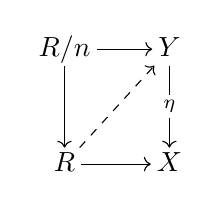
\begin{tikzpicture}[baseline=(current  bounding  box.center)]
\tikzstyle{every node}=[fill=white,  inner sep=2pt]
\matrix (m)
[	matrix of math nodes,
	row sep 		=	3em,
	column sep 	=	2em,
	text height	=	1.5ex,
	text depth	=	0.25ex
]
{ 		\Spec R/\fr{n}			&Y\\
		\Spec R					&X\\
};
\path[->, font=\scriptsize]
(m-1-1)	edge									(m-1-2)	
(m-1-1)	edge									(m-2-1)
(m-1-2)	edge node{$\eta$}				(m-2-2)
(m-2-1)	edge									(m-2-2);
\path[dashed, ->, font=\scriptsize]
(m-2-1)	edge									(m-1-2);
\end{tikzpicture}
\end{equation}
exist and commute, then the dashed arrow exists  (resp., is unique).
It is \emph{formally \'etale} iff it is both formally smooth and formally unramified.
We say that $\phi$ is \emph{smooth} (resp., \emph{unramified}, \emph{\'etale}) iff it is formally so, and moreover, of finite presentation.

These formal definitions are rather abstract.
Geometrically, $\Spec R/\fr{n} \to \Spec R$ is supposed to incarnate a ``thickening'' of $\Spec R/\fr{n}$ by ``tangent-vector data.''
The condition of $\eta$ being unramified (resp., smooth) means that tangency data at a point of $Y$ injects into (resp., surjects onto) tangency data at its image in $X$.
Thus, unramified (resp., smooth, \'etale) morphisms in algebraic geometry are the analogue of immersions (resp., submersions, local diffeomorphisms) in differential geometry.
Later, we will find that the analogy is most accurate when $\phi$ is a morphism of fg $k$-algebras for a field $k$.

\begin{prop}
If $\phi$ is a finite-type morphism between noetherian rings, then to check whether $\phi$ is smooth (resp., unramified, \'etale), it suffices to check those diagrams \eqref{SqZero} in which $R$ is local artinian.
\end{prop}

\subsubsection{Derivations and Differentials}

\newpage

%%%
\section{Sheaves}

\subsection{Quasicoherence}

\subsection{Flatness}

Flatness is a property of modules that corresponds roughly to the property of quasicoherent sheaves of restricting ``nicely'' to closed subschemes.
To be precise:

\begin{thm}
Let $M$ be an $A$-module.
Then the following are equivalent:
\begin{enumerate}
\item 	Tensoring with $M$ is an exact functor $\Mod_A \to \Mod_A$.
\item 	$\fr{a} \otimes M \simeq \fr{a}M$ for all $\fr{a} \normal A$.
\end{enumerate}
\end{thm}

\begin{rem}
Recall that tensoring with $M$ is \emph{always} a right-exact functor $\Mod_A \to \Mod_A$, because it is the left adjoint in the tensor-hom adjunction for $M$.
\end{rem}

\begin{proof}
If (1) holds, then $\fr{a} \otimes M \to A \otimes M \simeq M$ is injective, and we already know its image is $\fr{a}M$.
Conversely, suppose (2) holds.
We must show that if $N' \to N$ is an injection of $A$-modules, then $N' \otimes M \to N \otimes M$ remains an injection.
Since $N'$ is a colimit of fg $A$-modules and tensoring with $M$ is right-exact, we can assume $N'$ is fg.

\end{proof}

We say that $M$ is \emph{flat over $A$} iff it satisfies either of the equivalent conditions above.
We say that $M$ is \emph{faithfully flat over $A$} iff, more strongly, a sequence $N' \to N \to N''$ of $A$-modules is exact if and only if $N' \otimes M \to N \otimes M \to N'' \otimes M$ is exact.

\begin{prop}\mbox{}
\begin{enumerate}
\item 	A composition of flat (resp., faithfully flat) morphisms is flat (resp., faithfully flat).
\end{enumerate}
Let $\phi : A \to B$ be a ring morphism, and let $M$ be an $A$-module.
\begin{enumerate}\setcounter{enumi}{1}
\item 	If $\phi$ is flat and $M$ is flat over $A$, then $M \otimes_A B$ is flat over $B$.
\item 	If $\phi$ is faithfully flat, then $M$ is flat over $A$ if and only if $M \otimes_A B$ is flat over $B$.
\end{enumerate}
\end{prop}

\begin{prop}
Flatness can be checked on stalks.
\end{prop}

\begin{prop}
Let $M$ be an $A$-module.
\begin{enumerate}
\item 	If $M$ is projective, then $M$ is flat.
\item 	If $A$ is a PID, the $M$ is flat if and only if it is torsion-free.
\item 	If $M$ is finitely-presented, then $M$ is flat if and only if it is projective.
\item 	If $A$ is local and $M$ is finitely-presented, then $M$ is flat if and only if it is free.
\end{enumerate}
\end{prop}

\begin{proof}\mbox{}
\begin{enumerate}
\item 	
\item 	
\item 	
\item 	\qedhere
\end{enumerate}
\end{proof}

\subsubsection{The Topology of Flat Morphisms}

\begin{prop}
If $\phi : A \to B$ is a flat morphism, then $\phi$ satisfies the going-down property.
\end{prop}

\begin{prop}
Let $\phi : A \to B$ be a ring morphism.
Then $\phi$ is faithfully flat if and only if the induced map $\Spec B \to \Spec A$ is surjective.
\end{prop}

\begin{thm}
Let $\phi : A \to B$ be a local morphism of noetherian local rings.
If $\phi$ is flat and $\fr{m}_A$ is the maximal ideal of $A$, then 
\begin{align}
\dim B = \dim A + \dim B/\fr{m}_AB.
\end{align}
If $A$ is Cohen-Macaulay, then the converse holds.
\end{thm}

\subsection{Coherence}

\subsection{Freeness}


\begin{thm}[Generic Freeness]
Suppose $A$ is a noetherian domain and $A \to B$ is a finite morphism.
If $M$ is an fg $B$-module, then $M$ is free over $A$.
\end{thm}

\begin{cor}
Let $X = \Spec A$ and $Y = \Spec B$.
If $A$ is a noetherian domain and $f : Y \to X$ is a dominant morphism, then there exists open $U \subeq X$ such that $f^{-1}(\fr{p})$ has dimension $\dim Y - \dim X$ for all $\fr{p} \in U$.
\end{cor}

\subsection{Depth}

\subsection{Support and Annihilator}



%%%
%%%
%%%
\chapter{Schemes}

%%%
\section{Definition}

%%%
\section{Intrinsic Properties}

%%%
\section{Relative Properties}

%%%
\section{Sheaves}

%%%
\section{Differentials}

%%%
%%%
%%%
\chapter{Divisors}

%%%
\section{Cartier Divisors}

Let $X$ be a scheme.
For all open $U \subeq X$, let $S(U)$ be the multiplicative submonoid of $\cal{O}_X(U)$ of sections $s$ such that $s_x$ is not a zero-divisor in $\cal{O}_x$, for all $x \in U$.
The \emph{sheaf of total rings of fractions on $X$} is the sheafification $\cal{K}$ of the presheaf that sends $U \mapsto S(U)^{-1}$

%%%
\section{Weil Divisors}



%%%
\section{The Picard Group}

%%%
\section{The Grothendieck Group}

%%%
\section{Examples}





%%%
%%%
%%%
\chapter{Projective Schemes}

Throughout this chapter, let $R$ be a (nonnegatively) graded ring, i.e., 
\begin{align}
R = \bigoplus_{d \geq 0} R_d
\end{align}
and $\smash{R_{d_1} R_{d_2}} \subeq \smash{R_{d_1 + d_2}}$ for all $d_1, d_2$.
The Proj construction associates a scheme to $R$, denoted $\Proj R$, whose properties generalize those of projective spaces.
Indeed, if $k$ is a field and $R = k[t_0, \ldots, t_n]$ under the degree grading, then $\Proj R$ will be precisely the scheme associated to the classical projective $n$-space over $k$.

%%%
\section{Definition}

\subsection{}

Recall that if $M$ is a graded $R$-module, then a submodule $N$ of $M$ is said to be \emph{homogeneous} iff it can be generated by homogeneous elements, or equivalently, iff the following property holds:
For all $x  = \sum_d x_d \in M$, where $x_d \in M_d$, we have $x \in N$ if and only if $x_d \in N$ for all $d$.
If $N$ is an arbitrary submodule of $M$, then 
\begin{align}
N^\gr = \bigoplus_d~(N \cap R_d)
\end{align}
is the largest homogeneous submodule contained in $N$.
Taking $M = R$, we see this discussion applies to ideals.
The quotient of $R$ by a homogeneous ideal remains a graded ring in a canonical way.

Very roughly, homogeneous ideals are to $\Proj R$ what (ordinary) ideals are to $\Spec R$.

\begin{prop}\label{GradedPrime}
If $\fr{a} \normal A$ is homogeneous, then the following are equivalent:
\begin{enumerate}
\item 	$\fr{a}$ is a prime ideal.
\item 	For all homogeneous $f, g \in A$, we have $fg \in \fr{a}$ if and only if either $f \in\fr{a}$ or $g \in \fr{a}$.
\end{enumerate}
\end{prop}

\begin{proof}
If $\fr{a}$ is prime, then the conclusion of (2) holds even if $f, g$ are not homogeneous.
To prove (2) implies (1):
Suppose $f, g$ are elements, not necessarily homogeneous, such that $fg \in \fr{a}$.
Write $f = \sum_{n = 0}^r f_d$ and $g = \sum_{d = 0}^s g_d$, where $f_d, g_d \in A_d$.
After extending the sums by setting $f_d= 0$ for $d > r$ and $g_d = 0$ for $d > s$, we have $fg = \sum_{d = 0}^{r + s}~(f_0g_d + \cdots + f_dg_0)$.
We see $f_0g_0 = (fg)_0 \in \fr{a}$, whence either $f_0 \in \fr{a}$ or $g_0 \in \fr{a}$.
Now induct on $d$.
\end{proof}

\begin{cor}\label{Homogenizer}
If $\fr{p} \normal A$ is prime, then $\fr{p}^\gr$ is prime.
\end{cor}

\begin{proof}
By Prop.~\ref{GradedPrime}, it suffices to check that if $f,g\in A$ are homogeneous and $fg \in \fr{p}^\gr$, then either $f \in \fr{p}^\gr$ or $g \in \fr{p}^\gr$.
But $\fr{p}^\gr \subeq \fr{p}$, so the result follows from the primality of $\fr{p}$ and the definition of $\fr{p}^\gr$.
\end{proof}

We define the underlying set of $\Proj A$ to be the set of homogeneous prime ideals of $A$ that do not contain the so-called \emph{irrelevant ideal} $A_+ = \bigoplus_{n > 0} A_d$.

\begin{cor}\label{GradedNil}
$\nil A$ is the intersection of the homogeneous prime ideals of $A$.
Thus, $\Proj A$ is empty if and only if $\nil A \supseteq A_+$.
\end{cor}

\begin{proof}
Recall that $\nil A = \bigcap_{\fr{p} \in \Spec A} \fr{p}$.
We have inclusions
\begin{align}
\bigcap_{\fr{p} \in \Spec A} \fr{p}^\gr
\subeq 		\bigcap_{\fr{p} \in\Spec A} \fr{p} 
\subeq 		\bigcap_{\substack{\fr{p} \in \Spec A \\ \text{$\fr{p}$ homogeneous}}} \fr{p},
\end{align}
and the circle of inclusions is completed by Cor.~\ref{Homogenizer}.
In particular, $\fr{p} \supseteq A_+$ holds for all homogeneous prime ideals $\fr{p}$ if and only if $\nil A \supseteq A_+$.
\end{proof}

If $T \subeq A$ is an arbitrary subset, then we write $Z_+(T) = \{\fr{p} \in \Proj A : \fr{p} \supseteq T\}$.
If $f \in A_+$ is homogeneous, then we write $D_+(f) = (\Proj A) \setminus Z_+(\{f\})$.

\begin{prop}\label{GradedZariski}\mbox{}
\begin{enumerate}
\item 	If $T_1, \ldots, T_n \subeq A$, then $Z_+(T_1) \cup \cdots \cup Z_+(T_n) = Z_+(T_1 \cap \cdots \cap T_n) = Z_+(T_1\cdots T_n)$.
\item 	If $\{T_i\}_i$ is an arbitrary collection of subsets of $A$, then $\bigcap_i Z_+(T_i) = Z_+(\bigcup_i T_i)$.
\item 	If $f_1, \ldots, f_n \in A_+$ are homogeneous, then $D_+(f_1)\cap \cdots \cap D_+(f_n) = D_+(f_1 \cdots f_n)$.
\item 	\emph{Prime avoidance}.
			Suppose $\fr{a} \normal A$ is homogeneous and contained in $A_+$.
			If $\fr{p}_1, \ldots, \fr{p}_n \in \Proj A$ such that $\fr{p}_1, \ldots, \fr{p}_n \notin Z_+(\fr{a})$, then $\fr{p}_1, \ldots, \fr{p}_n \in D_+(f)$ for some $f \in \fr{a}$.
\end{enumerate}
\end{prop}

\begin{proof}\mbox{}
\begin{enumerate}
\item 	Follows from the affine version of this result.
\item 	By definition.
\item 	Follows from part (1).
\item 	By the affine version, we know that $\fr{p}_1, \ldots, \fr{p}_d \in D(f) \cap \Proj A$ for some $f \in \fr{a}$.
			Since $\fr{a}$ is homogeneous and contained in $A_+$, we know $f \in A_+$, and can assume $f$ is homogeneous, in which case $D(f) \cap \Proj A = D_+(f)$.
			\qedhere
\end{enumerate}
\end{proof}

By Prop.~\ref{GradedZariski}(1-2), we can define the \emph{Zariski topology} on $\Proj A$ to be the topology in which the closed sets take the form $Z_+(\fr{a})$ for homogeneous $\fr{a} \normal A$.
By Prop.~\ref{GradedZariski}(3), the sets $D_+(f)$ form a basis of open neighborhoods as $f$ runs through homogeneous elements in $A_+$; once again, they are called \emph{distinguished opens}.

\subsection{}

Before defining the structure sheaf of $\Proj A$, we need some notation regarding localization in graded rings.
If $T$ is a (multiplicative) submonoid of $A$, then the set $T_+$ of homogeneous elements of $T$ forms a further submonoid.
If $M$ is a graded $A$-module, then the \emph{homogeneous localization of $M$ at $T$} is $(T_+^{-1}M)_0$, the $A_0$-module of fractions expressible in the form $x/f$ for some homogeneous $x \in M$ and $f \in T_+$ of the same degree.
If $T = A \setminus \fr{p}$ for some $\fr{p} \in \Proj A$ (resp., if $T = \{f^n\}_{n = 0}^\infty$ for some homogeneous $f \in A_+$), then we denote this module by $M_{(\fr{p})}$ (resp., $M_{(f)}$).
A homogeneous localization of a graded $A$-algebra is again a graded $A$-algebra in a canonical way.

%		The \emph{$d$th Veronese subring} of $A$ is the graded ring $\smash{A^{(d)}}$ formed by $A$ under the grading
%		\begin{align}
%		A^{(d)}_d = A_{dn}.
%		\end{align}

We define $\cal{O}_{\Proj A}$ to be the sheafification of  the ring-valued presheaf on $\Proj A$ that sends an open $U$ to the homogeneous localization of $A$ at  $\bigcap_{\fr{p} \in U}~(A \setminus \fr{p})$.
Explicitly, a section of $\cal{O}_{\Proj A}$ over $U$ is a right inverse $s$ of the projection $\coprod_{\fr{p} \in U} A_{(\fr{p})} \to U$, such that for all $\fr{p} \in U$, we can find open $V \subeq U$ containing $\fr{p}$ and homogeneous $f, g \in A$ of the same degree, satisfying $g \notin \fr{q}$ and $s(\fr{q}) = f/g$ for all $\fr{q} \in V$.
Thus, we have the following characterization of stalks and sections over distinguished opens for $\Proj A$:

\begin{prop}\mbox{}
\begin{enumerate}
\item 	$\cal{O}_{\Proj A, \fr{p}} \simeq A_{(\fr{p})}$ for all $\fr{p} \in \Proj A$.
\item 	$\cal{O}_{\Proj A}(D_+(f)) \simeq A_{(f)}$ for all homogeneous $f \in A_+$.
\end{enumerate}
\end{prop}

\begin{cor}
$(D_+(f), \cal{O}_{\Proj A}|_{D_+(f)}) \simeq \Spec A_{(f)}$ for all homogeneous $f \in A_+$.
\end{cor}

\begin{cor}
$\Proj A$ is a scheme.
If $k$ is a field and $A$ is the homogeneous coordinate ring of a variety $V$ over $k$, then $\Proj A$ is the scheme associated to $V$.
\end{cor}

\begin{ex}
If $S$ is an arbitary scheme, then we define the (scheme-theoretic) \emph{projective $n$-space over $S$} to be the fiber product
\begin{align}
\bb{P}_S^n = \Proj \bb{Z}[t_0, \ldots, t_n] \times_{\bb{Z}} S.
\end{align}
If $S = \Spec \cal{O}$, then we instead write $\smash{\bb{P}_{\cal{O}}^n}$.

In parallel with the classical setting, $\smash{\bb{P}_{\cal{O}}^n}$ has a canonical affine open cover $\smash{\{D_+(t_i)\}_{i = 0}^n}$, where $D_+(t_i) \simeq \smash{\bb{A}_\cal{O}^n}$ as an open subscheme of $\smash{\bb{P}_\cal{O}^n}$ via the explicit isomorphism:
\begin{align}
\cal{O}[s_0, \ldots, \hat{s}_i, \ldots, s_n] 
&\simeq 	\cal{O}[t_0, \ldots, t_n]_{(t_i)} \\
f(s_0, \ldots, s_n) 
&\mapsto 	\smash{t_i^{\deg f}} 
					f(t_0/t_i, \ldots,  t_n/t_i),\nn
g(s_0, \ldots, 1, \ldots, s_n)
&\mapsfrom	g(t_0, \ldots, t_n)	\n
\end{align}
Above, the forward map is called \emph{homogenization} and the backward map is called \emph{dehomogenization}.
\end{ex}


%%%
\section{Sheaves}

%%%
\section{Morphisms to Projective Space}




%%%
%%%
%%%
\chapter{The Cohomology of Schemes}



%--------------------------------------------------------------------------

\backmatter

\begin{thebibliography}{.....  ..}
\bibitem[AM]{AM}
	M.\ Atiyah and I.\ G.\ Macdonald.
	\emph{Introduction to Commutative Algebra}.
	Addison-Wesley Publishing Company
	(1969).
	
\bibitem[EH]{EH}
	D.\ Eisenbud \& J.\ Harris.
	\emph{The Geometry of Schemes}.
	Springer-Verlag
	(2000).
	
\bibitem[Ha]{Ha}
	R.~Hartshorne.
	\emph{Algebraic Geometry}.
	Springer-Verlag
	(1977).
	
\bibitem[Ma]{Ma}
	H.~Matsumura.
	\emph{Commutative Ring Theory}.
	Trans.~M.~Reid.
	Cambridge University Press
	(2006).
	
\bibitem[SP]{SP}
	The Stacks Project Authors.
	\emph{Stacks Project}.
	(2014).
	\href{http://stacks.math.columbia.edu}{http://stacks.math.columbia.edu}
\end{thebibliography}

\end{document}